\documentclass[10pt,a4paper]{article}
\usepackage[T1]{fontenc}
\usepackage{lmodern,microtype}
\usepackage[margin=16mm,top=14mm,bottom=17mm]{geometry}
\usepackage{booktabs,tabularx,array}
\usepackage{tikz}
\usetikzlibrary{arrows.meta}
\usepackage{xcolor,hyperref,fancyhdr}
\definecolor{ink}{HTML}{17324D}
\definecolor{accent}{HTML}{216E72}
\hypersetup{colorlinks=true,urlcolor=accent,linkcolor=ink,pdftitle={Junco versus the Wavestone harness study},pdfauthor={Architecture comparison}}
\pagestyle{fancy}\fancyhf{}
\fancyfoot[L]{\scriptsize\color{ink}Junco / harness architecture audit}
\fancyfoot[R]{\scriptsize\thepage\ / 2}
\renewcommand{\headrulewidth}{0pt}
\setlength{\parindent}{0pt}
\setlength{\parskip}{4pt}
\setlength{\tabcolsep}{5pt}
\newcommand{\heading}[1]{\par\vspace{5pt}{\large\bfseries\color{ink}#1}\par\vspace{2pt}}
\newcommand{\src}[1]{\textcolor{accent}{\scriptsize[#1]}}
\newcommand{\pathref}[1]{{\ttfamily\scriptsize\detokenize{#1}}}
\newcolumntype{Y}{>{\raggedright\arraybackslash}X}
\tikzset{box/.style={draw=ink!65,rounded corners=1.5pt,align=center,minimum height=10mm,text width=33.5mm,inner sep=3pt,font=\fontsize{8.5}{10}\selectfont},flow/.style={-{Latex[length=1.6mm]},draw=ink!80,line width=.55pt},proposed/.style={box,draw=accent,dashed},note/.style={font=\fontsize{8}{9.5}\selectfont,align=center,text=ink!90}}
\begin{document}
{\LARGE\bfseries\color{ink}Junco versus the Wavestone harness study}\par
{\large Operational gaps in large-scale agentic programming}\par
{\small 24 October 2026\quad\textbullet\quad Source baseline: \texttt{3a5b73a03fa4}\quad\textbullet\quad Architecture, not a performance ranking}

\textbf{Assessment.} Junco is a capable local orchestration substrate, but unattended, long-running coding campaigns need guarantees that its components do not yet compose into a run-wide contract: restart recovery, bounded spending, containment, and verified publication. More agents alone will not close those gaps.

\textbf{Comparison basis.} Barbaste, Darrigol, Vu and Wiltberger's Wavestone/Inclusive Brains study surveys eleven harnesses and uses Omnigent as a meta-harness contrast. Its seven subsystems are loop, LLM integration, tools, context, safety, orchestration and extensibility [P, \S2.3]. It does not benchmark them [P, \S15.6]. This audit reads Junco's working-tree implementation; current Pi is \texttt{0.99.2}, not the paper's \texttt{0.80.6} snapshot. Risks and proposed changes below are architectural inferences, not measured failure rates.

\heading{What Junco already provides}
Recursive graphs and dynamic tasks sit above Pi's model/tool loop. Typed routes, stale-attempt rejection, cancellation/drain, model-strength ladders, context compaction, skills/hooks and managed MCP already exist. Marsh provides ownership-aware file/shell operations and workspace publication; optional cgroups constrain command pipelines. Calling Junco ``without memory, MCP or sandboxing'' would misidentify the problem.\src{A,B,D,E}

\begin{center}
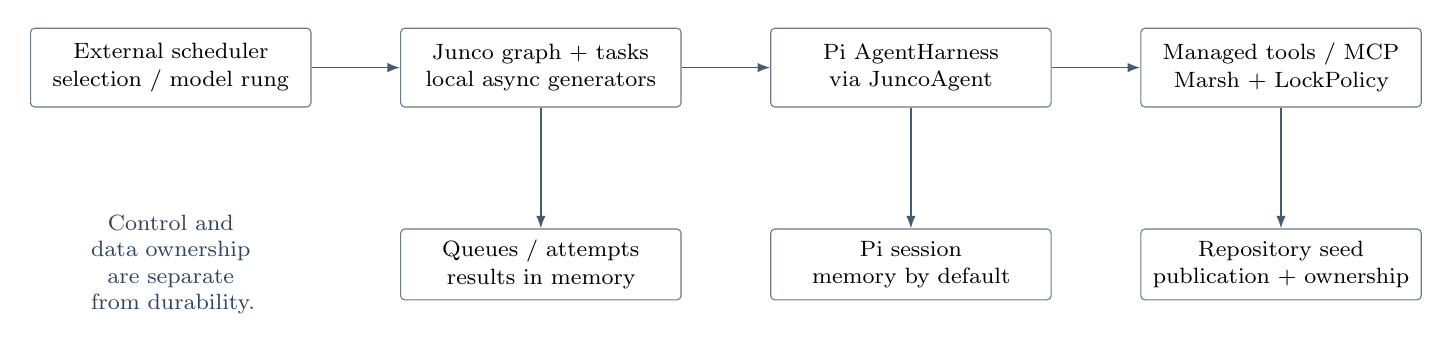
\begin{tikzpicture}[x=1mm,y=1mm]
\node[box] (sched) at (18,26) {External scheduler\\selection / model rung};
\node[box] (graph) at (65,26) {Junco graph + tasks\\local async generators};
\node[box] (agent) at (112,26) {Pi AgentHarness\\via JuncoAgent};
\node[box] (tools) at (159,26) {Managed tools / MCP\\Marsh + LockPolicy};
\node[box,minimum height=9mm] (state) at (65,1) {Queues / attempts\\results in memory};
\node[box,minimum height=9mm] (session) at (112,1) {Pi session\\memory by default};
\node[box,minimum height=9mm] (seed) at (159,1) {Repository seed\\publication + ownership};
\draw[flow] (sched)--(graph);\draw[flow] (graph)--(agent);\draw[flow] (agent)--(tools);
\draw[flow] (graph)--(state);\draw[flow] (agent)--(session);\draw[flow] (tools)--(seed);
\node[note,text width=34mm] at (18,1) {Control and data ownership\\are separate from durability.};
\end{tikzpicture}
\end{center}
\vspace{-5pt}
{\small\textbf{Figure 1.} Current control path, simplified. A root may receive a durable Pi session; created children use memory sessions. Arbitrary caller tools are a separate trusted execution path, not automatically Marsh-managed.\src{A,B,D}}

\heading{The consequential shortfalls}
{\small
\renewcommand{\arraystretch}{1.12}
\begin{tabularx}{\linewidth}{@{}>{\raggedright\arraybackslash}p{27mm}Y@{}}
\toprule
\textbf{Gap / priority} & \textbf{Current boundary and why it matters}\\
\midrule
Restart and retry\newline\textbf{P0} & Junco rejects a supplied session with an open operation (\texttt{cannot attach to an open operation}); every spawned child gets a fresh \texttt{MemorySessionRepo}. Graph queues and attempts are also local. A retry starts a fresh child with the same prompt, not a durable side-effect transaction. Pi transcripts alone cannot recover a campaign. Contrast OpenHands's event log and OpenCode's persisted work queue [P, \S6.2].\src{A,B}\\
\addlinespace[3pt]
Containment and policy\newline\textbf{P0} & Workspace snapshots are explicitly \emph{not OS confinement}. Exact collection tools get owner-bound execution; arbitrary tools execute caller code. Parent hooks are not inherited by children. Therefore file ownership and a parent approval hook do not establish fleet-wide filesystem, credential or network policy. Compare Codex's OS/policy stack [P, \S10.2; recommendation 10].\src{B,D}\\
\addlinespace[3pt]
Run-wide budgets\newline\textbf{P0} & The scheduler limits \emph{predicted column memory}, excluding memory retained across yields. Token/cost thresholds notify a callback; they do not themselves reject the next request. Optional cgroups limit individual pipelines, not aggregate LLM spending or all host memory. Recursive fan-out needs one shared accounting/admission boundary [P, \S6.2; recommendation 18].\src{B,C,D}\\
\addlinespace[3pt]
Accepted code\newline\textbf{P1} & Generic task completion tests \texttt{stopReason == stop}, not compilation or tests. Yak Shaver already demonstrates deterministic review/application gates, but these are workflow-specific. Direct seed reads can observe multi-file publication in progress. Acceptance must name the \emph{exact artifact} checked, rather than infer correctness from task settlement [P, \S6.3, \S11.4].\src{A,D,F}\\
\bottomrule
\end{tabularx}}

\textbf{Scale boundary.} Selected work currently advances local promises and drains an entire column before replanning; lane limits are not remote workers or failover. Introduce worker leases and recovery only when jobs must outlive or exceed one host. Per-agent tools are also forced sequential, so independent reads lose concurrency; measure that bottleneck before adding more agents. ACP is an outward hosting seam [P, recommendation 13], not a prerequisite for internal scheduling. Do not add a new framework or vector database merely to match the paper's inventory [P, recommendations 8, 15--16].\src{A,B}

\newpage
\heading{Close the guarantees before expanding the fleet}
\textbf{First: make recovery an explicit protocol.} Reuse Pi's existing open-operation and lane-resume APIs instead of rejecting interrupted sessions. Allow a durable child-session factory; journal task identity, attempt, delivered inputs and published artifact IDs. Checkpoint at explicit task boundaries, not by serializing JavaScript generators. Give non-idempotent effects operation IDs and recorded outcomes; an ambiguous external write must require reconciliation before replay.\src{A,B,G}

\textbf{Then: bind admission and acceptance to those identities.} Add a shared run ledger for reserved/actual tokens, dollars, deadlines and live resources across roots, retries and descendants. Enforce it before provider/tool admission; notification remains useful for reporting. Supply a production profile with configured cgroups, a scrubbed environment and actual OS confinement. Explicit caller tools remain trusted host code unless isolated; install policy on every child at construction, not only on its parent.\src{B,C,D}

\begin{center}
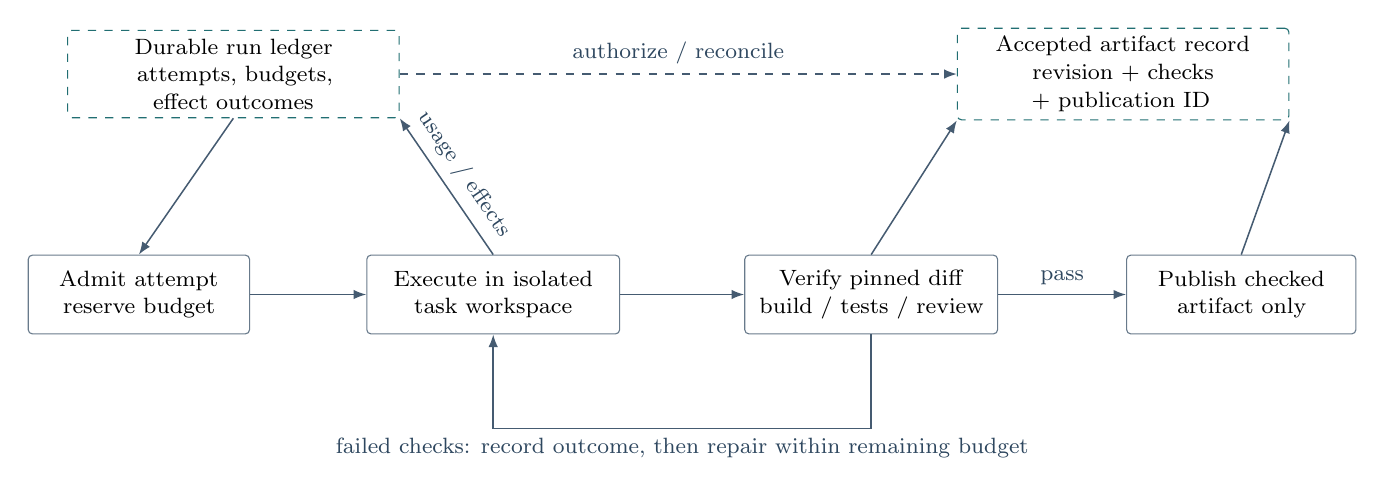
\begin{tikzpicture}[x=1mm,y=1mm]
\node[proposed,text width=40mm] (ledger) at (28,43) {Durable run ledger\\attempts, budgets, effect outcomes};
\node[proposed,text width=40mm] (journal) at (141,43) {Accepted artifact record\\revision + checks + publication ID};
\node[box,text width=26mm] (admit) at (16,15) {Admit attempt\\reserve budget};
\node[box,text width=30mm] (work) at (61,15) {Execute in isolated\\task workspace};
\node[box,text width=30mm] (verify) at (109,15) {Verify pinned diff\\build / tests / review};
\node[box,text width=27mm] (publish) at (156,15) {Publish checked\\artifact only};
\draw[flow] (admit)--(work);\draw[flow] (work)--(verify);\draw[flow] (verify)--node[above,note]{pass}(publish);
\draw[flow] (ledger.south)--(admit.north);
\draw[flow] (verify.north)--(journal.south west);
\draw[flow] (publish.north)--(journal.south east);
\draw[flow] (work.north)--node[above,sloped,note]{usage / effects}(ledger.south east);
\draw[flow] (verify.south)--(109,-2)--node[below,note]{failed checks: record outcome, then repair within remaining budget}(61,-2)--(work.south);
\draw[flow,dashed] (ledger.east)--node[above,note]{authorize / reconcile}(journal.west);
\end{tikzpicture}
\end{center}
\vspace{-5pt}
{\small\textbf{Figure 2.} Proposed acceptance/recovery contract, \emph{not current implementation}. Dashed boxes are durable additions; ordinary boxes reuse Junco's scheduler, task, deterministic-node and tool seams. Recovery must consult effect outcomes before retrying; telemetry is a separate observer, not the commit log.}

\textbf{Keep verification in the graph.} Use deterministic sink/finalization nodes, following Yak Shaver, to require fresh machine-checkable evidence for the candidate revision. Serialize or isolate integration until the checked diff can be published without changing its meaning. Record rejection as a normal outcome; do not replace compilation/tests with an LLM's statement that they passed. Hermes's verify-on-stop and OpenHands's outer judge illustrate the stop boundary [P, \S6.2, \S11.4]; neither substitutes for an artifact-specific test result.\src{A,D,F}


\textbf{Evidence to require before calling this production-ready.} Kill/restart between tool effect and acknowledgement; demonstrate reconciliation without duplicate publication. Run concurrent children against one token/dollar ceiling and show denied admission. Reject a failed build against a pinned revision. Exercise an untrusted tool's host-path/network denial. These are proposed acceptance checks, \emph{not results of this audit}.

{\small\textbf{Observed smoke scope.} The offline recursive-agent example completed with \texttt{leaf-result + sibling-result} and 16 root decisions. The memory-limit example emitted seven scheduling columns under declared profiles. These exercise local composition and predictive admission, not crash recovery, containment or large-scale throughput. Commands from the repository root:\\
\pathref{bun run examples/recursive-agency/recursive-agency.ts}\\
\pathref{bun run packages/dataflow-engine/examples/memory-limit.ts}}

\heading{Sources and reproducibility}
{\fontsize{8}{9.4}\selectfont
\textbf{[P]} P. Barbaste et al., \emph{Harness Engineering: Anatomy, Architecture, and Evolution of Coding Agents---A Source-Code Study of Eleven Systems}, arXiv:2609.00006v1. \href{https://arxiv.org/abs/2609.00006}{Abstract/PDF}; \href{https://arxiv.org/html/2609.00006v1}{section-addressable full text}. Paper claims are attributed, not independently replicated.\\[2pt]
\textbf{Repository:} \href{https://github.com/junco-org/junco-agency/tree/3a5b73a03fa49f08f5ce9d2f97d88f2f315fa462}{junco-org/junco-agency, base revision \texttt{3a5b73a03fa4}}; local paths/line spans below.\\
Path prefixes: \texttt{J=packages/junco-agent}, \texttt{T=packages/junco-tools},\\
\texttt{E=packages/dataflow-engine}, \texttt{S=packages/junco-scheduler}.\\[2pt]
\textbf{[A]} \pathref{E/src/dataflow-graph.ts:184-205,619-654}; \pathref{src/agent-node.ts:393-412,770-794}.\\
\textbf{[B]} \pathref{J/src/junco-agent.ts:769-811,839-858,1028-1044,1688-1701}; \pathref{J/README.md:99-123}.\\
\textbf{[C]} \pathref{S/src/resources.ts:100-143}. \textbf{[D]} \pathref{T/ts/operations.ts:30-40}; \pathref{T/README.md:83-91,324-350}.\\
\textbf{[E]} \pathref{src/junco-graph.ts:418-488}; installed Pi \texttt{0.99.2}, \pathref{dist/harness/compaction/compaction.js:74-79} (auto-compaction).\\
\textbf{[F]} \pathref{examples/yak-shaver/yak-shaver.ts:1249-1256,1296-1344}.\\
\textbf{[G]} installed \texttt{@earendil-works/pi-agent-core@0.99.2}, \pathref{dist/harness/agent-harness.d.ts:155-161,647-657,706-710} (open operations/resume).\\[2pt]
\textbf{Audit limit:} static code comparison plus the two offline examples; no live-model benchmark, crash-injection experiment or OS-confinement test. Opik export is best-effort, not durable recovery evidence: \pathref{packages/dataflow-engine-opik/src/opik-tracer.ts:77-82,177-182}.
}
\end{document}
